\PassOptionsToPackage{unicode}{hyperref}
\documentclass[t]{beamer}

\usepackage[
  orientation=portrait,
  size=a0,
  scale=1.0,
]{beamerposter}

\usetheme{tudoposter}

\usepackage{fontspec}

%\usepackage{polyglossia}
%\setmainlanguage{german}
\usepackage[english]{babel}

\usepackage{csquotes}
\usepackage{microtype}
\usepackage{mathtools}

\usepackage{blindtext}

\usepackage{multicol}
\setlength{\columnsep}{1em}

\usepackage{xfrac}

\usepackage{tikz}
\usetikzlibrary{shapes, arrows, backgrounds, fit, tikzmark, arrows.meta, calc, quotes, angles}

\usepackage[center]{caption}

\usepackage{siunitx}

\usepackage[export]{adjustbox}

\usepackage{xcolor}
\usepackage{listings}
\lstset{
  commentstyle=\color{black!60},    % comment style
}

\lstdefinestyle{base}{
  moredelim=**[is][\color{black!30}]{@}{@},
}

\usepackage{mdframed} %nice frames
\definecolor{light-gray}{gray}{0.95} %the shade of grey that stack exchange uses

\usepackage{graphicx}

%% this is used to create an inline bibliography
\usepackage[backend=biber, style=numeric]{biblatex}
\addbibresource{biblatex-phys.bib}

\DeclareFieldFormat*{title}{\textit{#1}}
\renewcommand*{\bibfont}{\footnotesize}
\defbibenvironment{bibliography}
  {\noindent}
  {\unspace}
  {}

\renewbibmacro*{begentry}{%
  \usebeamercolor{bibliography item}%
  \color{bibliography item.fg}%
  \printtext[labelnumberwidth]{%
    \printfield{prefixnumber}%
    \printfield{labelnumber}%
  }%
  \setunit{\addnbspace}%
}
\renewcommand*{\finentrypunct}{\addperiod\space}

\newlength{\thirdtextwidth}
\setlength\thirdtextwidth{0.333333\textwidth}

\newlength{\itemseparation}
\setlength\itemseparation{0.25em}

\title{High-energy lepton and photon propagation with the simulation framework PROPOSAL}
\author{Jean-Marco Alameddine$^{1}$, Alexander Sandrock$^{2}$, Wolfgang Rhode$^{1}$, Jan Soedingrekso$^{1}$}
\institute[ETH]{$^{1}$TU Dortmund University, Otto-Hahn-Str. 4a, 44227 Dortmund, Germany \\$^{2}$University of Wuppertal, Gaußstraße 20, 42119 Wuppertal, Germany}
\date{4. Juli 2015}

\titlegraphic{%
  
\includegraphics[width=1.0\linewidth, left]{tudo.pdf}\\
  \vspace{0.2em}
  
\includegraphics[width=0.8\linewidth, left]{BUW.png}\\
  %\vspace{0.2em}
  %
\includegraphics[width=1.0\linewidth, left]{dfg_logo_englisch_blau_en.jpg}
}

\begin{document}
      \begin{block}[equal height group=A]{Introduction}%
        \setlength{\columnsep}{40pt} 
        \begin{multicols}{2}
          \begin{itemize}
            \setlength\itemsep{\itemseparation}
            \item PROPOSAL is a C\texttt{++}/Python \textbf{simulation framework}, providing 3D Monte Carlo simulations of high-energy electrons, positrons, muons, taus and photons \cite{koehne2013proposal, dunsch_2018_proposal_improvements}
            \item Different parametrizations of physical processes, including up-to-date parametrizations, are available
            \item Customizable propagation environment
            \item High-performance and high-precision simulations, optimized for long-scale particle propagation
          \end{itemize}
          
          \vspace{-1.5em}
    \centering
    \captionof*{figure}{Basic propagation algorithm of PROPOSAL:}
    \begin{minipage}{0.7\linewidth}
    \begin{columns}
        \begin{column}{0.3\textwidth}
        \centering
        \colorbox{light-gray}{
      \begin{minipage}{6.0cm}
          \centering
        $\underset{\text{relative energy loss}}{v}$
    \end{minipage}
      }        
      \end{column}

        \begin{column}{0.1\textwidth}
          with
        \end{column}
        \begin{column}{0.3\textwidth}
        \centering
        \colorbox{cyan}{
      \begin{minipage}{6.0cm}
        \centering
        $\underset{\text{continuous losses}}{v < v_\text{cut}}$
    \end{minipage}
      }
        \end{column}

        \begin{column}{0.3\textwidth}
        \centering
        \colorbox{orange}{
      \begin{minipage}{6.0cm}
          \centering
        $\underset{\text{stochastic losses}}{v > v_\text{cut}}$
    \end{minipage}
      }
        \end{column}
    \end{columns}
    \end{minipage}

    \vspace{-3em}


  \centering
    \begin{tcolorbox}[colback=light-gray,colframe=black,width=0.8\linewidth]
    \begin{figure}
      \normalsize
      \begin{tikzpicture}[scale=2.50]
        \centering
            \coordinate (E0) at (0,0);
            \coordinate (E1) at (1/3 * 10, -1/3 * 1);
            \coordinate (E2) at (2/3 * 10, -2/3 * 1);
            \coordinate (E3) at (10, -1);

      \draw [cyan, line width=0.6mm] (E0) -- (E1) node[pos=0.5, sloped, above] {$E_i^0 \rightarrow E_f^0$};
      \draw [cyan, line width=0.6mm] (E1) -- (E2) node[pos=0.5, sloped, above] {$E_i^1 \rightarrow E_f^1$};
      \draw [cyan, line width=0.6mm] (E2) -- (E3) node[pos=0.5, sloped, above] {$E_i^2 \rightarrow E_f^2$};

      \fill [black] (E0) circle (0.15) node[label=below: $E_{i}^0$]{};
      \fill [orange] (E1) circle (0.15) node[label=below: $\color{black} E_{f}^0 (1 - \textcolor{orange}{v_0}) \equiv E_i^1$]{};
      \fill [orange] (E2) circle (0.15) node[label=below: $\color{black} E_{f}^1 (1 - \textcolor{orange}{v_1}) \equiv E_i^2$]{};
      \fill [black] (E3) circle (0.15) node[label=below: $\color{black} E_{f}^2$]{};


      \end{tikzpicture}
    \end{figure}
    \end{tcolorbox}
    \vspace{-3em}
    \begin{minipage}{0.9\linewidth}
    \Large
    \begin{columns}[onlytextwidth]
      \begin{column}{0.5\textwidth}  
        \centering
        $\displaystyle\int_{E_i}^{E_f} \frac{\sigma\left(E\right)}{-f\left(E\right)} \cdot \mathrm{d}E = -\log{\left( \xi \right)}$
      \end{column}
      \begin{column}{0.5\textwidth}
        \centering
        $v_\text{cut} = \text{min}\left[\sfrac{e_\text{cut}}{E}, v\prime_\text{cut}\right]$  
      \end{column}
    \end{columns}
    \end{minipage}



          \columnbreak
          \begin{multicols}{2}
            \begin{figure}
              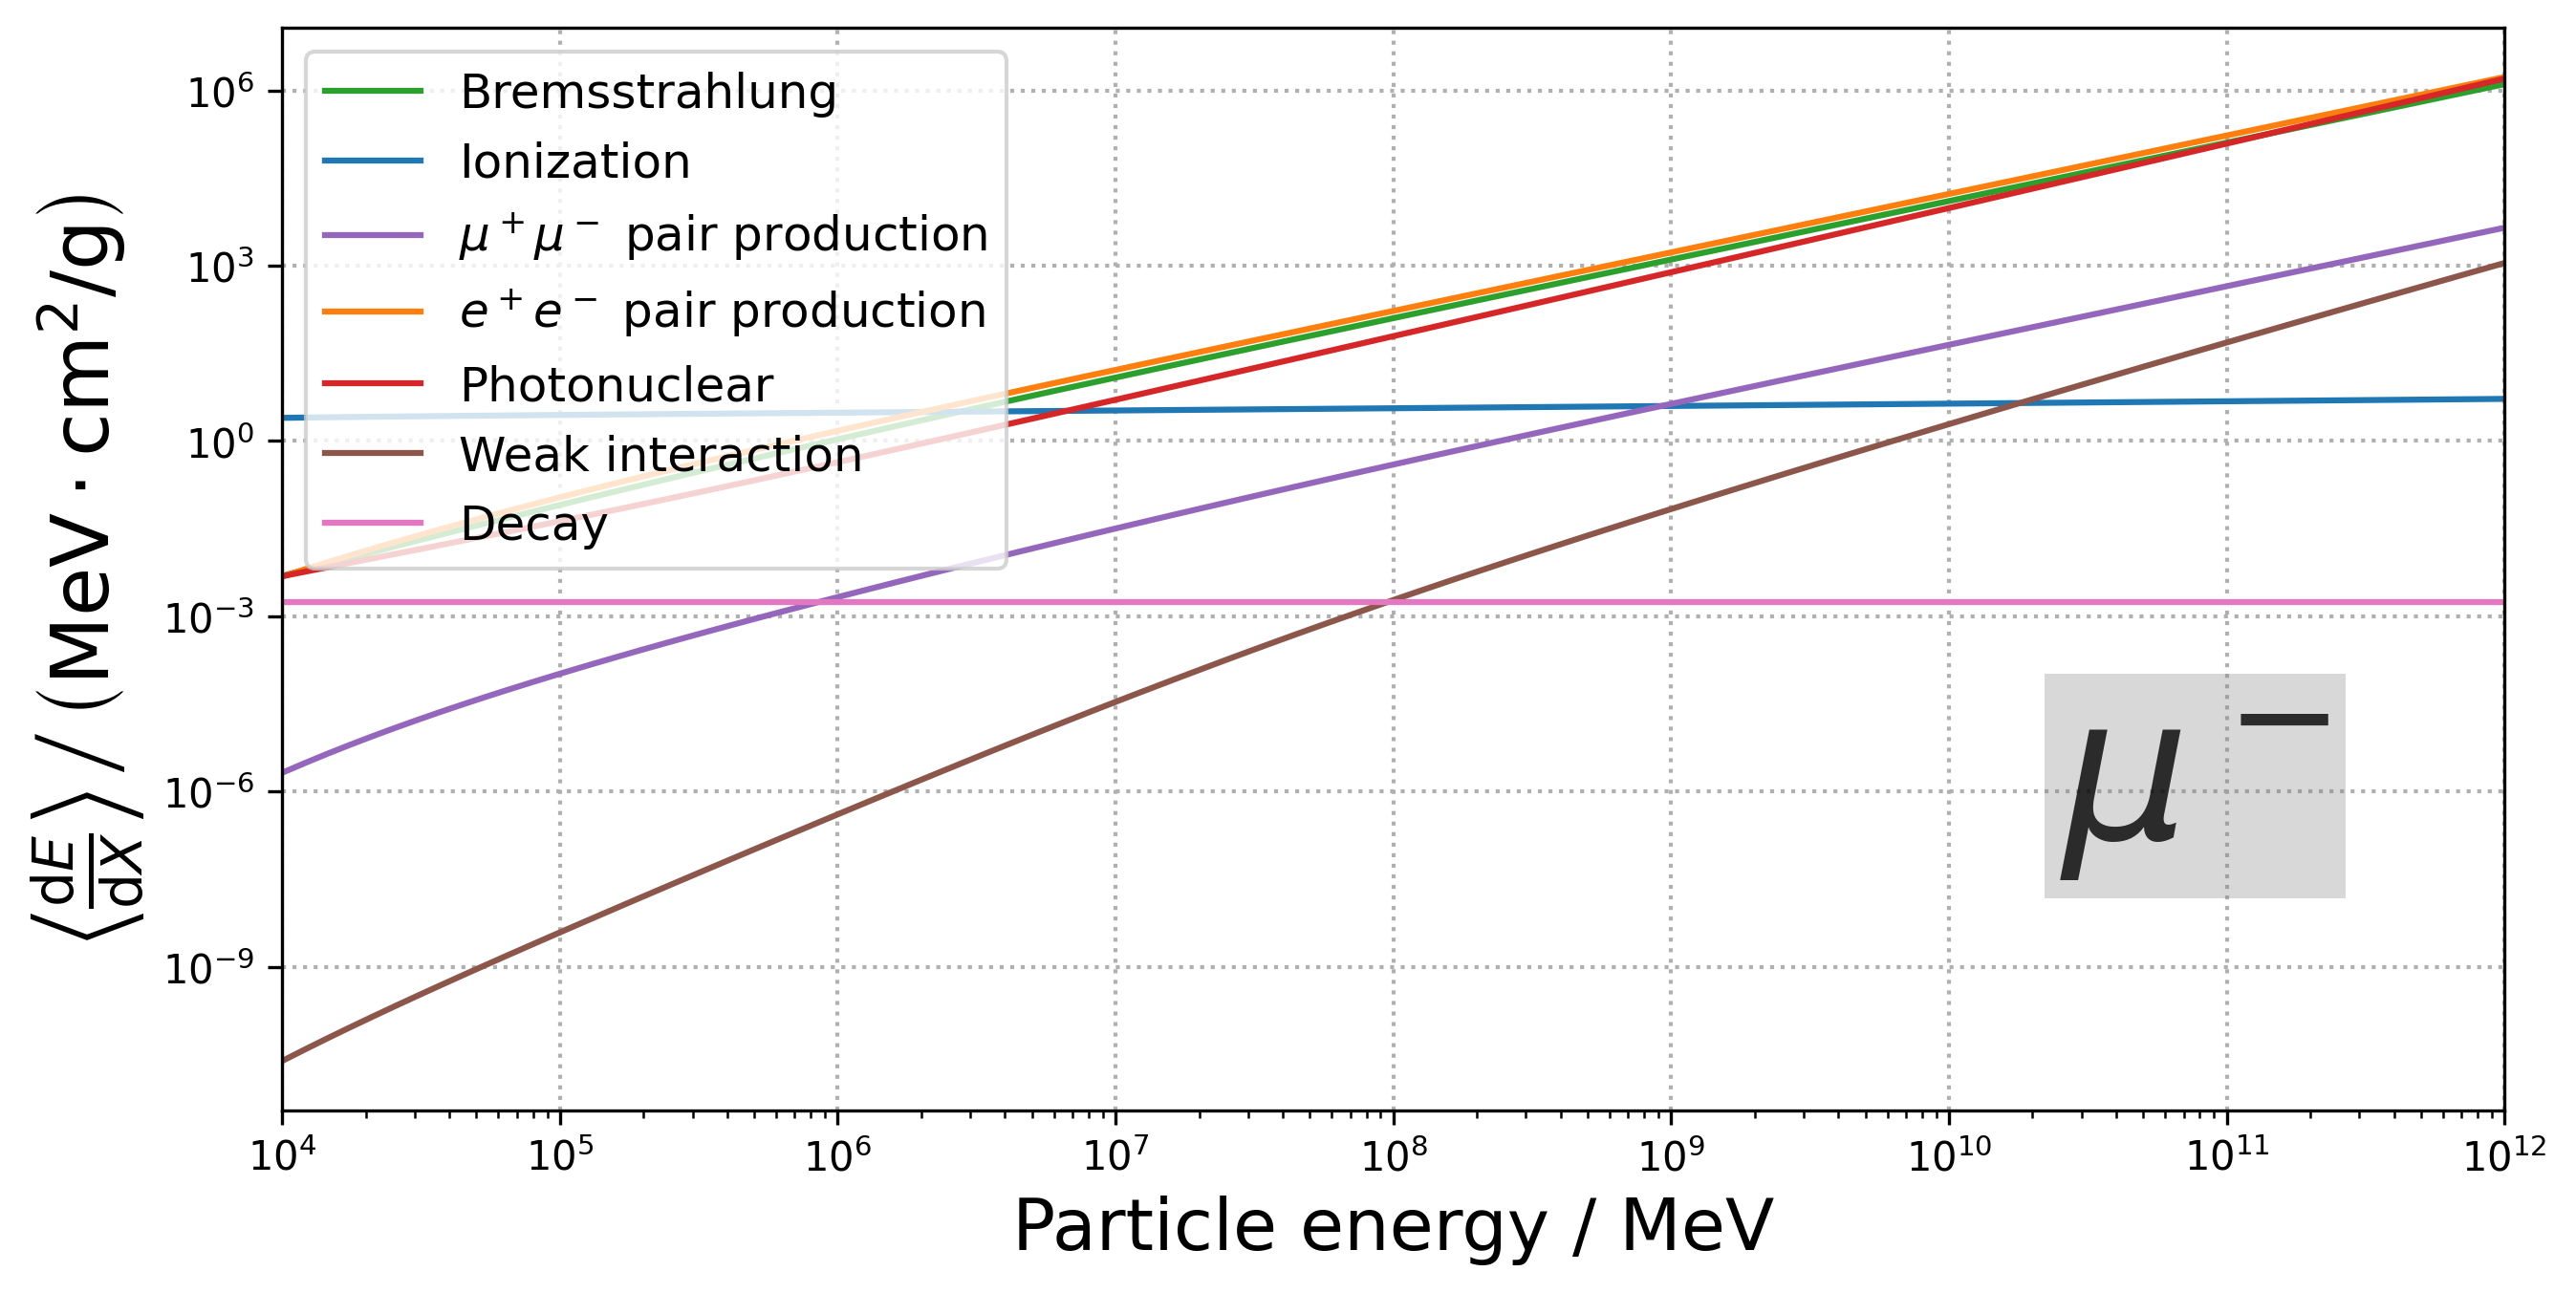
\includegraphics[width=\linewidth, height=.4\textheight, keepaspectratio]{plots/muon_dEdx.png}
            \end{figure}
            \begin{figure}
              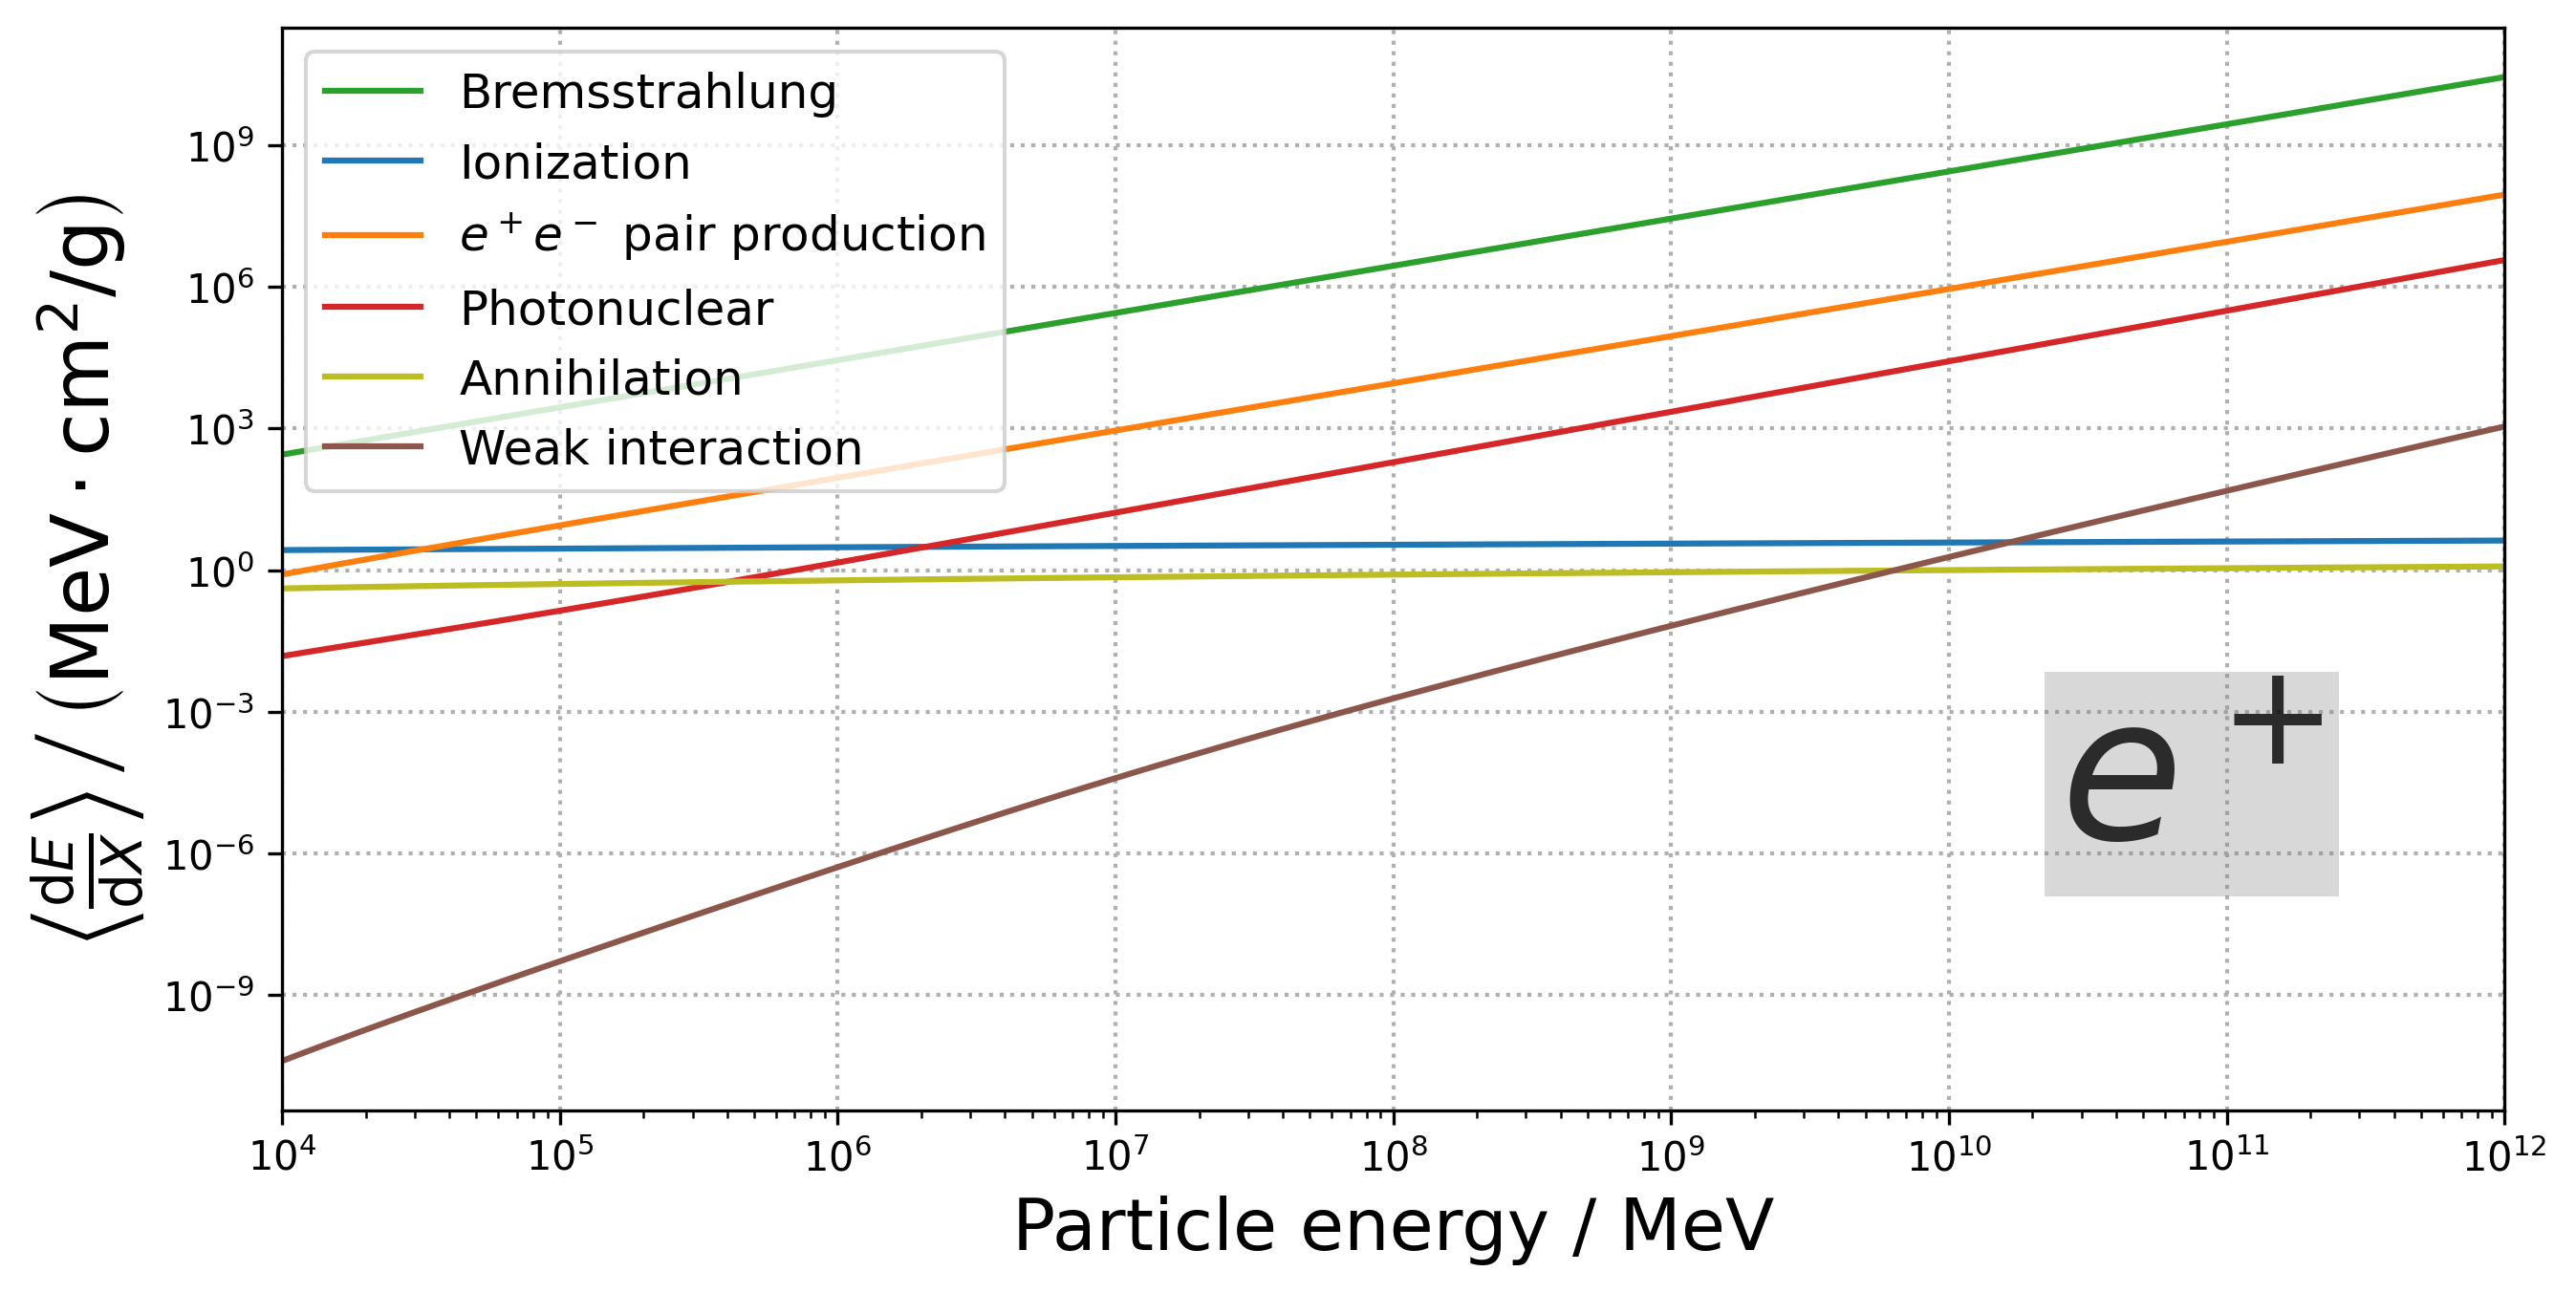
\includegraphics[width=\linewidth, height=.4\textheight, keepaspectratio]{plots/positron_dEdx.png}
            \end{figure}
            \columnbreak
            \begin{figure}
              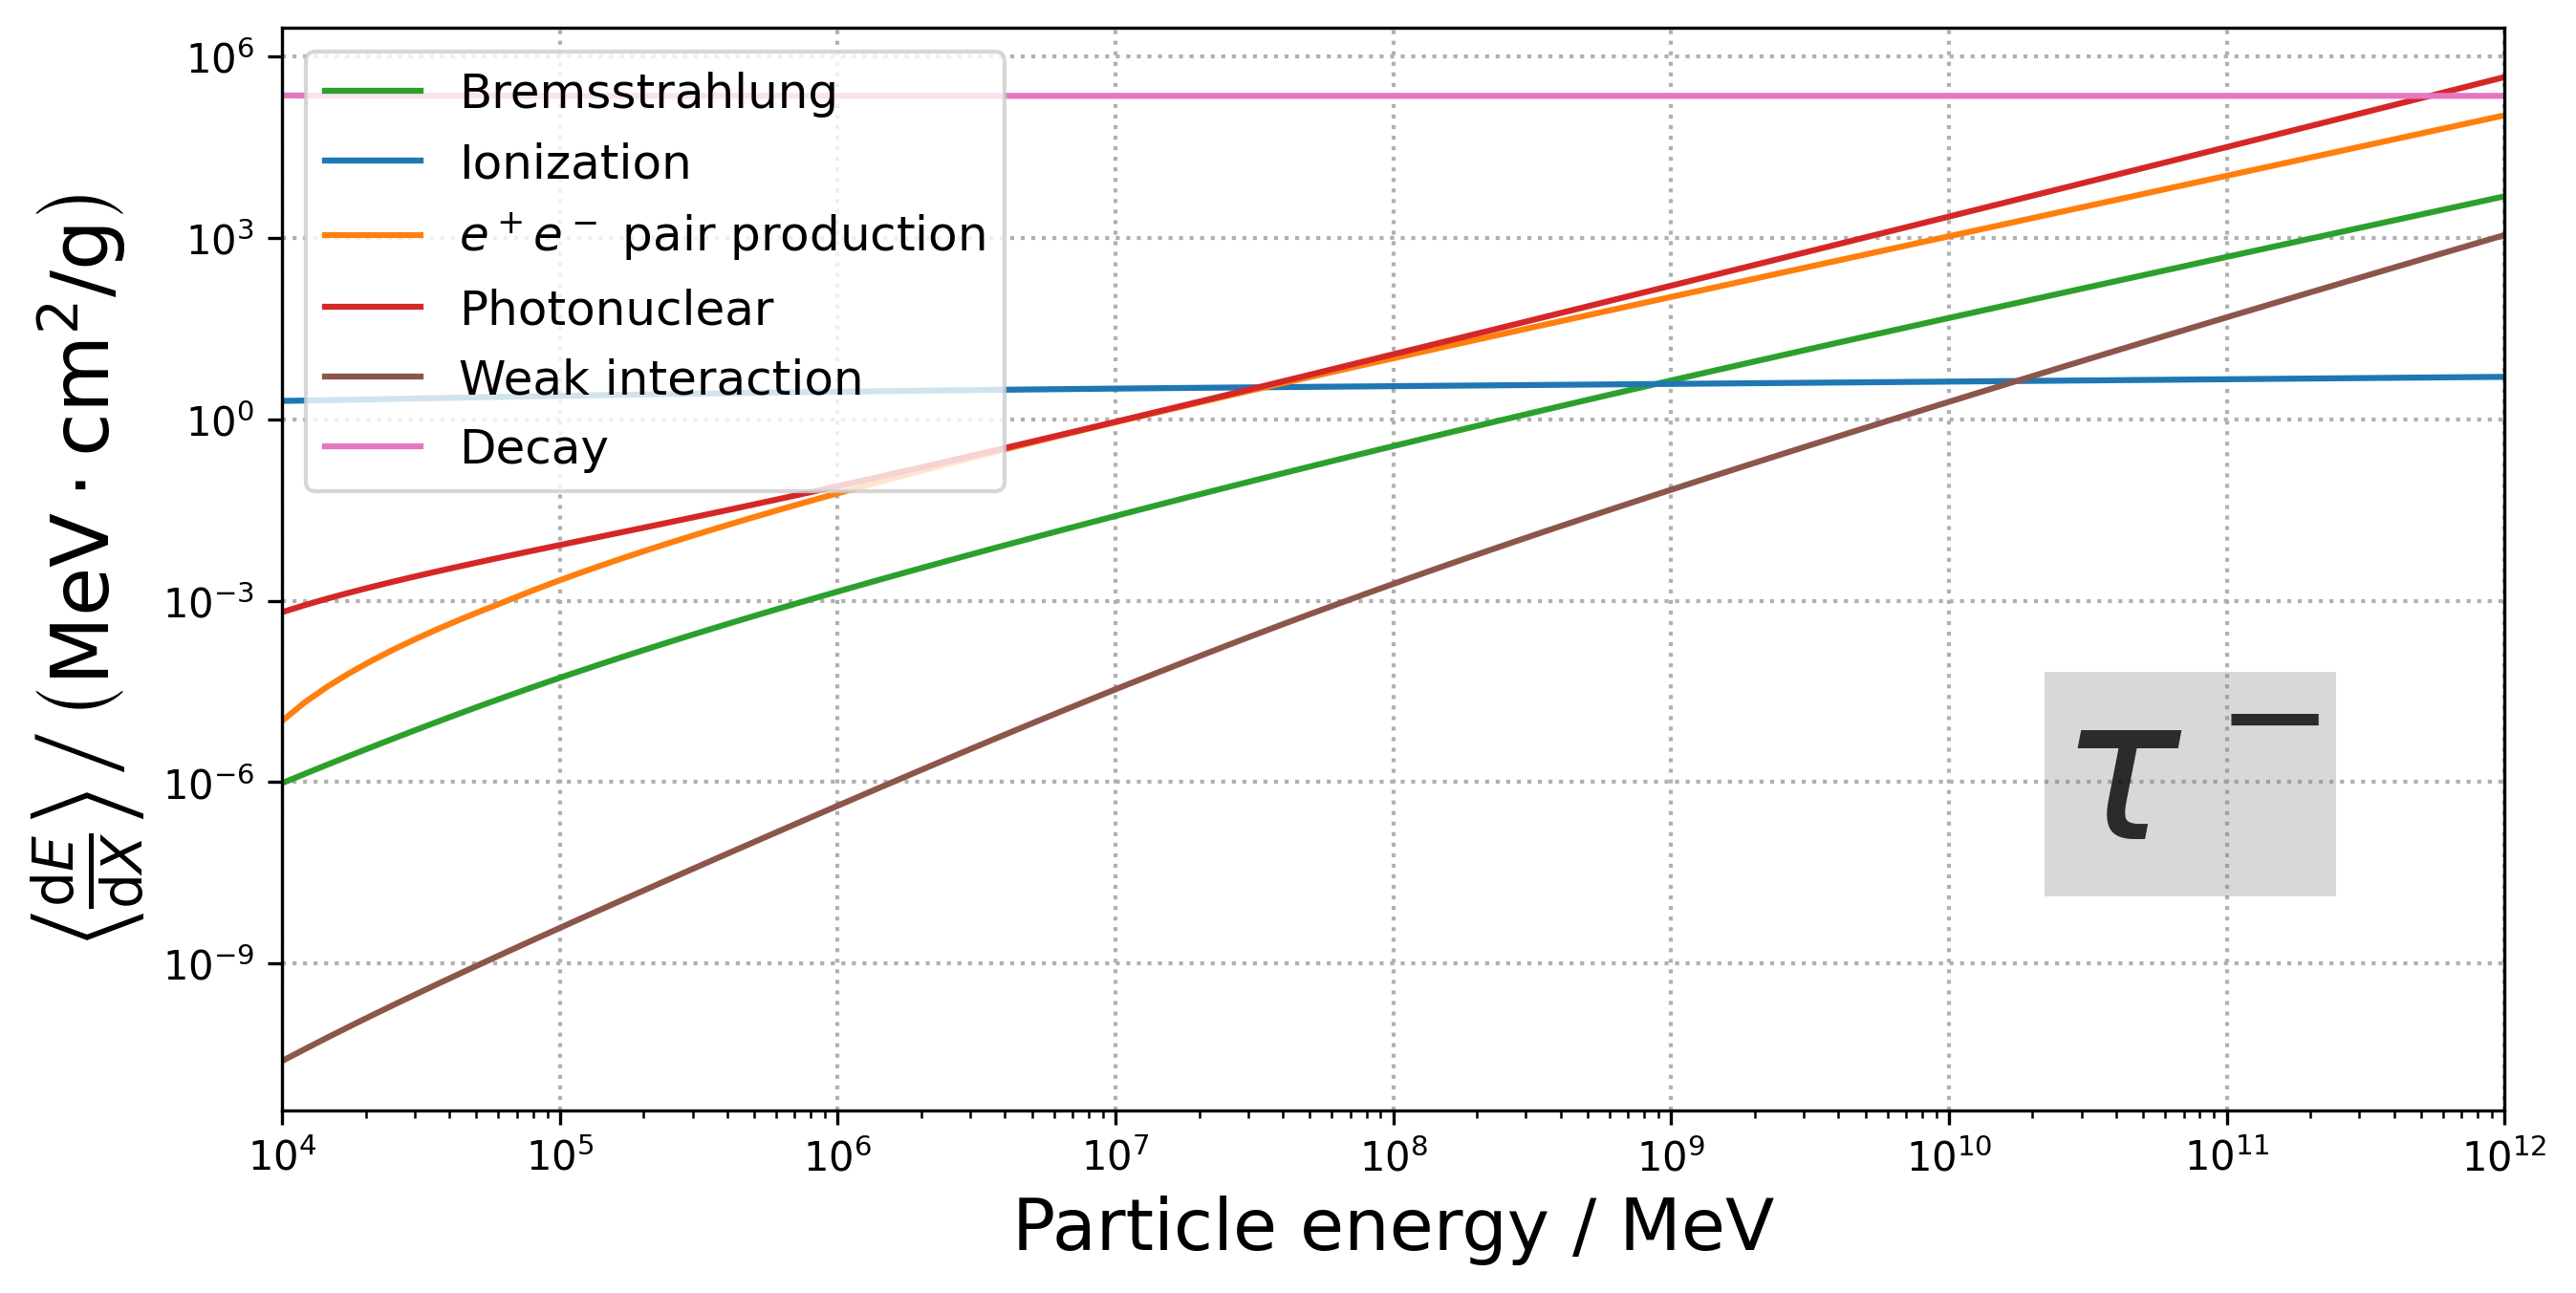
\includegraphics[width=\linewidth, height=.4\textheight, keepaspectratio]{plots/tau_dEdx.png}
            \end{figure}
            \begin{figure}
              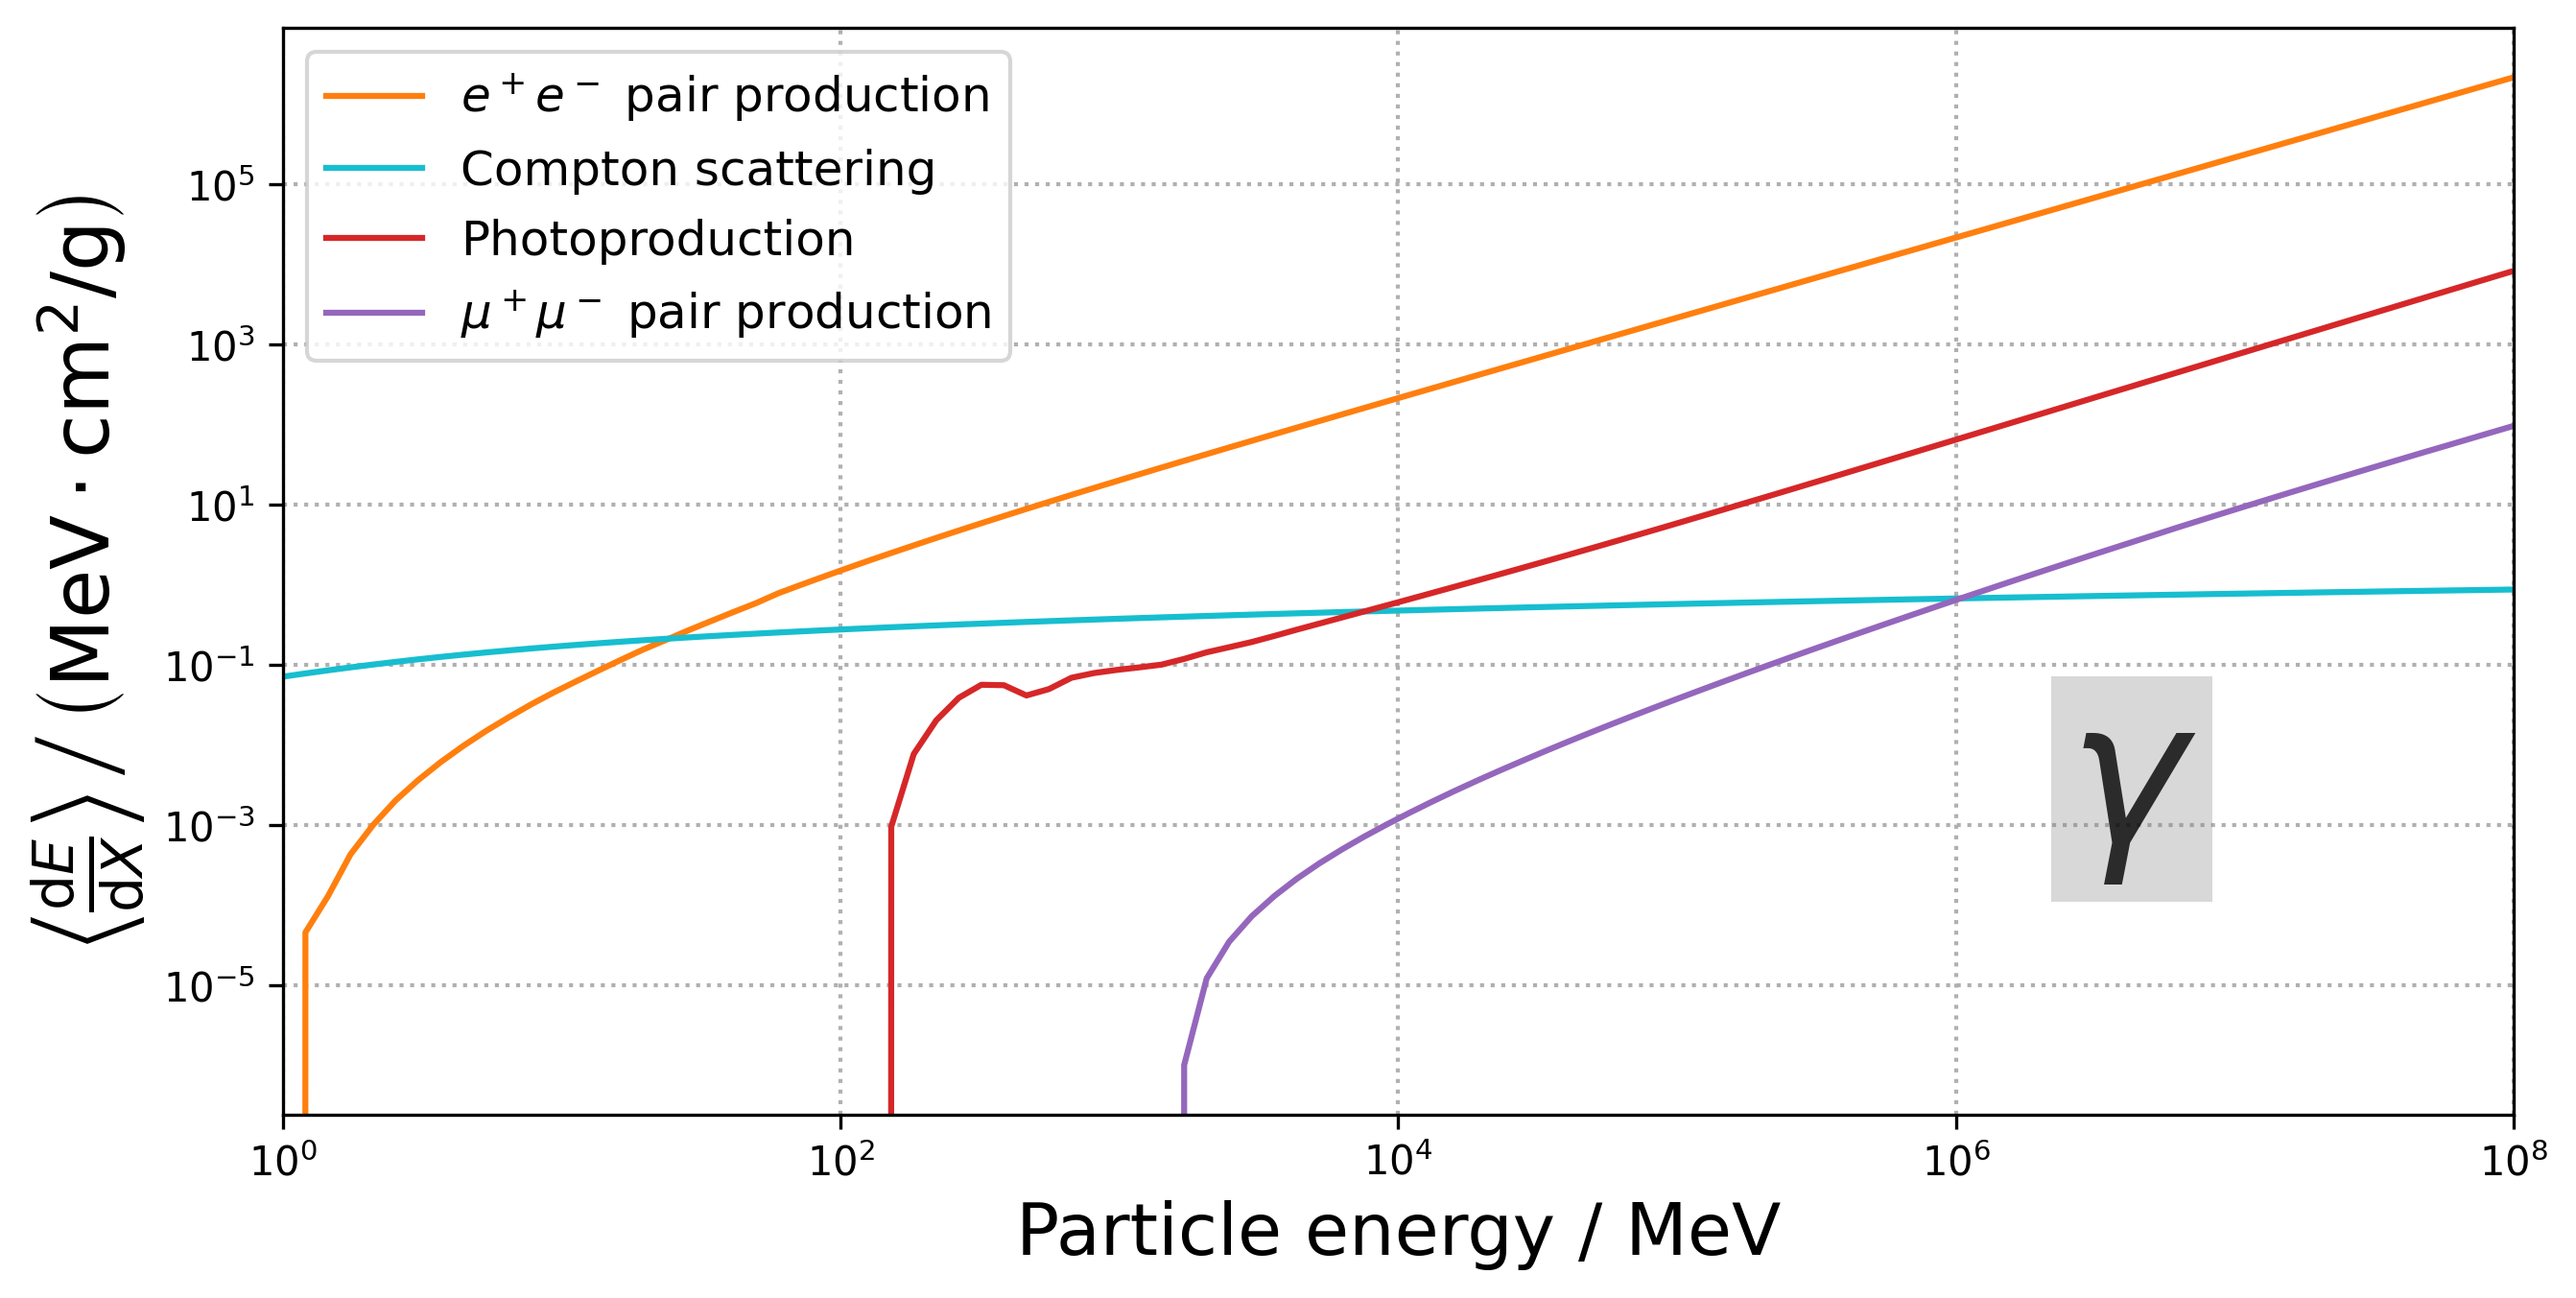
\includegraphics[width=\linewidth, height=.4\textheight, keepaspectratio]{plots/photon_dEdx.png}
            \end{figure}
          \end{multicols}
           \captionof*{figure}{Average energy losses of particles inside PROPOSAL.}

        \end{multicols}
      \end{block}%
  \begin{columns}[onlytextwidth]%
    \begin{column}{0.6\textwidth}%
      \begin{block}{How to use PROPOSAL}%
        \begin{itemize}
          \setlength\itemsep{\itemseparation}
          \item PROPOSAL can be used as a C\texttt{++} or a Python library
            \begin{itemize}
              \setlength\itemsep{\itemseparation}
              \item[$\rightarrow$] Simple installation with \texttt{pip install proposal}
            \end{itemize}
          \item Information about the configuration environment can be read using a json file
        \end{itemize}

        \begin{columns}[onlytextwidth]
        \begin{column}{0.45\textwidth}
        \begin{mdframed}[backgroundcolor=light-gray, roundcorner=10pt,leftmargin=1, rightmargin=1, innerleftmargin=15, innertopmargin=15,innerbottommargin=15, outerlinewidth=1, linecolor=light-gray]

          \lstinputlisting[
          language=Python,
          basicstyle=\footnotesize\ttfamily,
          style=base,
          escapechar=\$,
          breaklines=true
          ]{code/example.txt}
          \end{mdframed} 

          \end{column}
          \begin{column}{0.1\textwidth}
          \begin{center}
            \vspace{7em}
            \begin{tikzpicture}
            \draw[
              -triangle 90,
               line width=4mm,
                postaction={draw, line width=0.7cm, shorten >=1cm, -}
            ] (0,0) -- (2,0);
          \end{tikzpicture}
          \end{center}          
        \end{column}
          \begin{column}{0.45\textwidth}
            \begin{figure}
              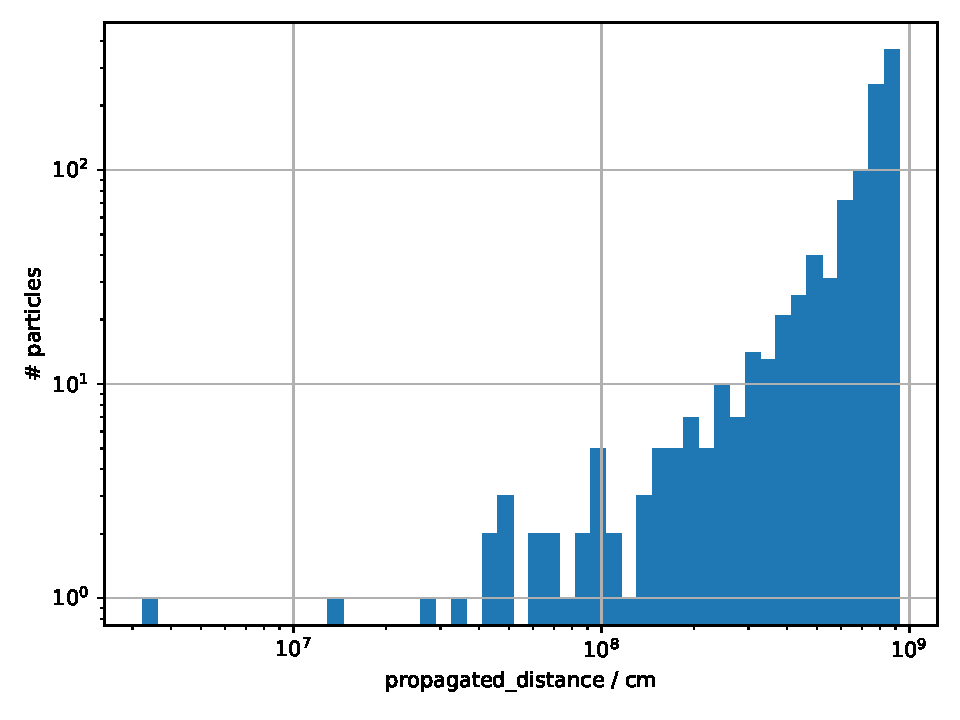
\includegraphics[width=\linewidth, height=.4\textheight, keepaspectratio]{plots/example_output.pdf}
            \end{figure}
          \end{column}
        \end{columns}

      \end{block}%
    \end{column}%
    \begin{column}{0.4\textwidth}%
      \begin{block}{Recent updates of PROPOSAL}%
        PROPOSAL is updated regularly. Recent improvements include:
        \begin{itemize}
          \setlength\itemsep{\itemseparation}
          \item Simulation of stochastic deflections, i.e. deflection of particles in hard losses
          \item Additions of new $\gamma$ effects
          \begin{itemize}
            \setlength\itemsep{\itemseparation}
            \item[$\rightarrow$] $\gamma \rightarrow \text{Hadron}$ interactions
            \item[$\rightarrow$] $\gamma \rightarrow \mu^+ \mu^-$
            \item[$\rightarrow$] Analytical description of the photoeffect
          \end{itemize}
        \end{itemize}
      \end{block}%
    \end{column}%
  \end{columns}%
  \begin{columns}[onlytextwidth]%
    \begin{column}{0.6\textwidth}%
      \begin{block}[equal height group=B]{Application: CORSIKA~8}%
          \begin{columns}[onlytextwidth]  
            \begin{column}{0.6\textwidth}%
              \begin{itemize}
                \setlength\itemsep{\itemseparation}
                \item CORSIKA~8 is the newest version of the air shower simulation framework CORSIKA
                \begin{itemize}
                  \setlength\itemsep{\itemseparation}
                  \item[$\rightarrow$] Entirely new code structure, based on modern C\texttt{++} 
                  \item[$\rightarrow$] Focus on flexibilty, modularity, efficiency and reliability \cite{Engel2018}
                \end{itemize}
                \item For CORSIKA~8, PROPOSAL is used to simulate the electromagnetic and muonic shower component
                \begin{itemize}
                  \setlength\itemsep{\itemseparation}
                  \item[$\rightarrow$] PROPOSAL provides individual modules, where each module solves specific physical tasks \cite{Alameddine_2020}
                  \item[$\rightarrow$] CORSIKA~8 uses these modules to calculate interaction lengths, energy losses and multiple scattering 
                \end{itemize}
                \item First comparisons of CORSIKA~8 and CORSIKA~7 already show a good agreement for simulations of the electromagnetic shower component \cite{Alameddine:2021iq}
              \end{itemize}

\vspace{2em}
\begin{center}
        \colorbox{light-gray}{
      \begin{minipage}{0.85\linewidth}


\begin{figure}[ht]
\begin{minipage}[ht]{0.58\linewidth}
Find the CORSIKA~8 repository under:\\ \url{gitlab.iap.kit.edu/AirShowerPhysics/corsika}
\end{minipage}
%\begin{minipage}[ht]{0.05\linewidth}
%\end{minipage}
\begin{minipage}[ht]{0.41\linewidth}
\centering

\includegraphics[%scale=1
                 width=0.8\linewidth, valign=t]{plots/qr_corsika_transparent.png}
\end{minipage}
\end{figure}

    \end{minipage}
      }    

\end{center}

            \end{column}
            \begin{column}{0.4\textwidth}%
              \centering
              \begin{figure}
                \centering
                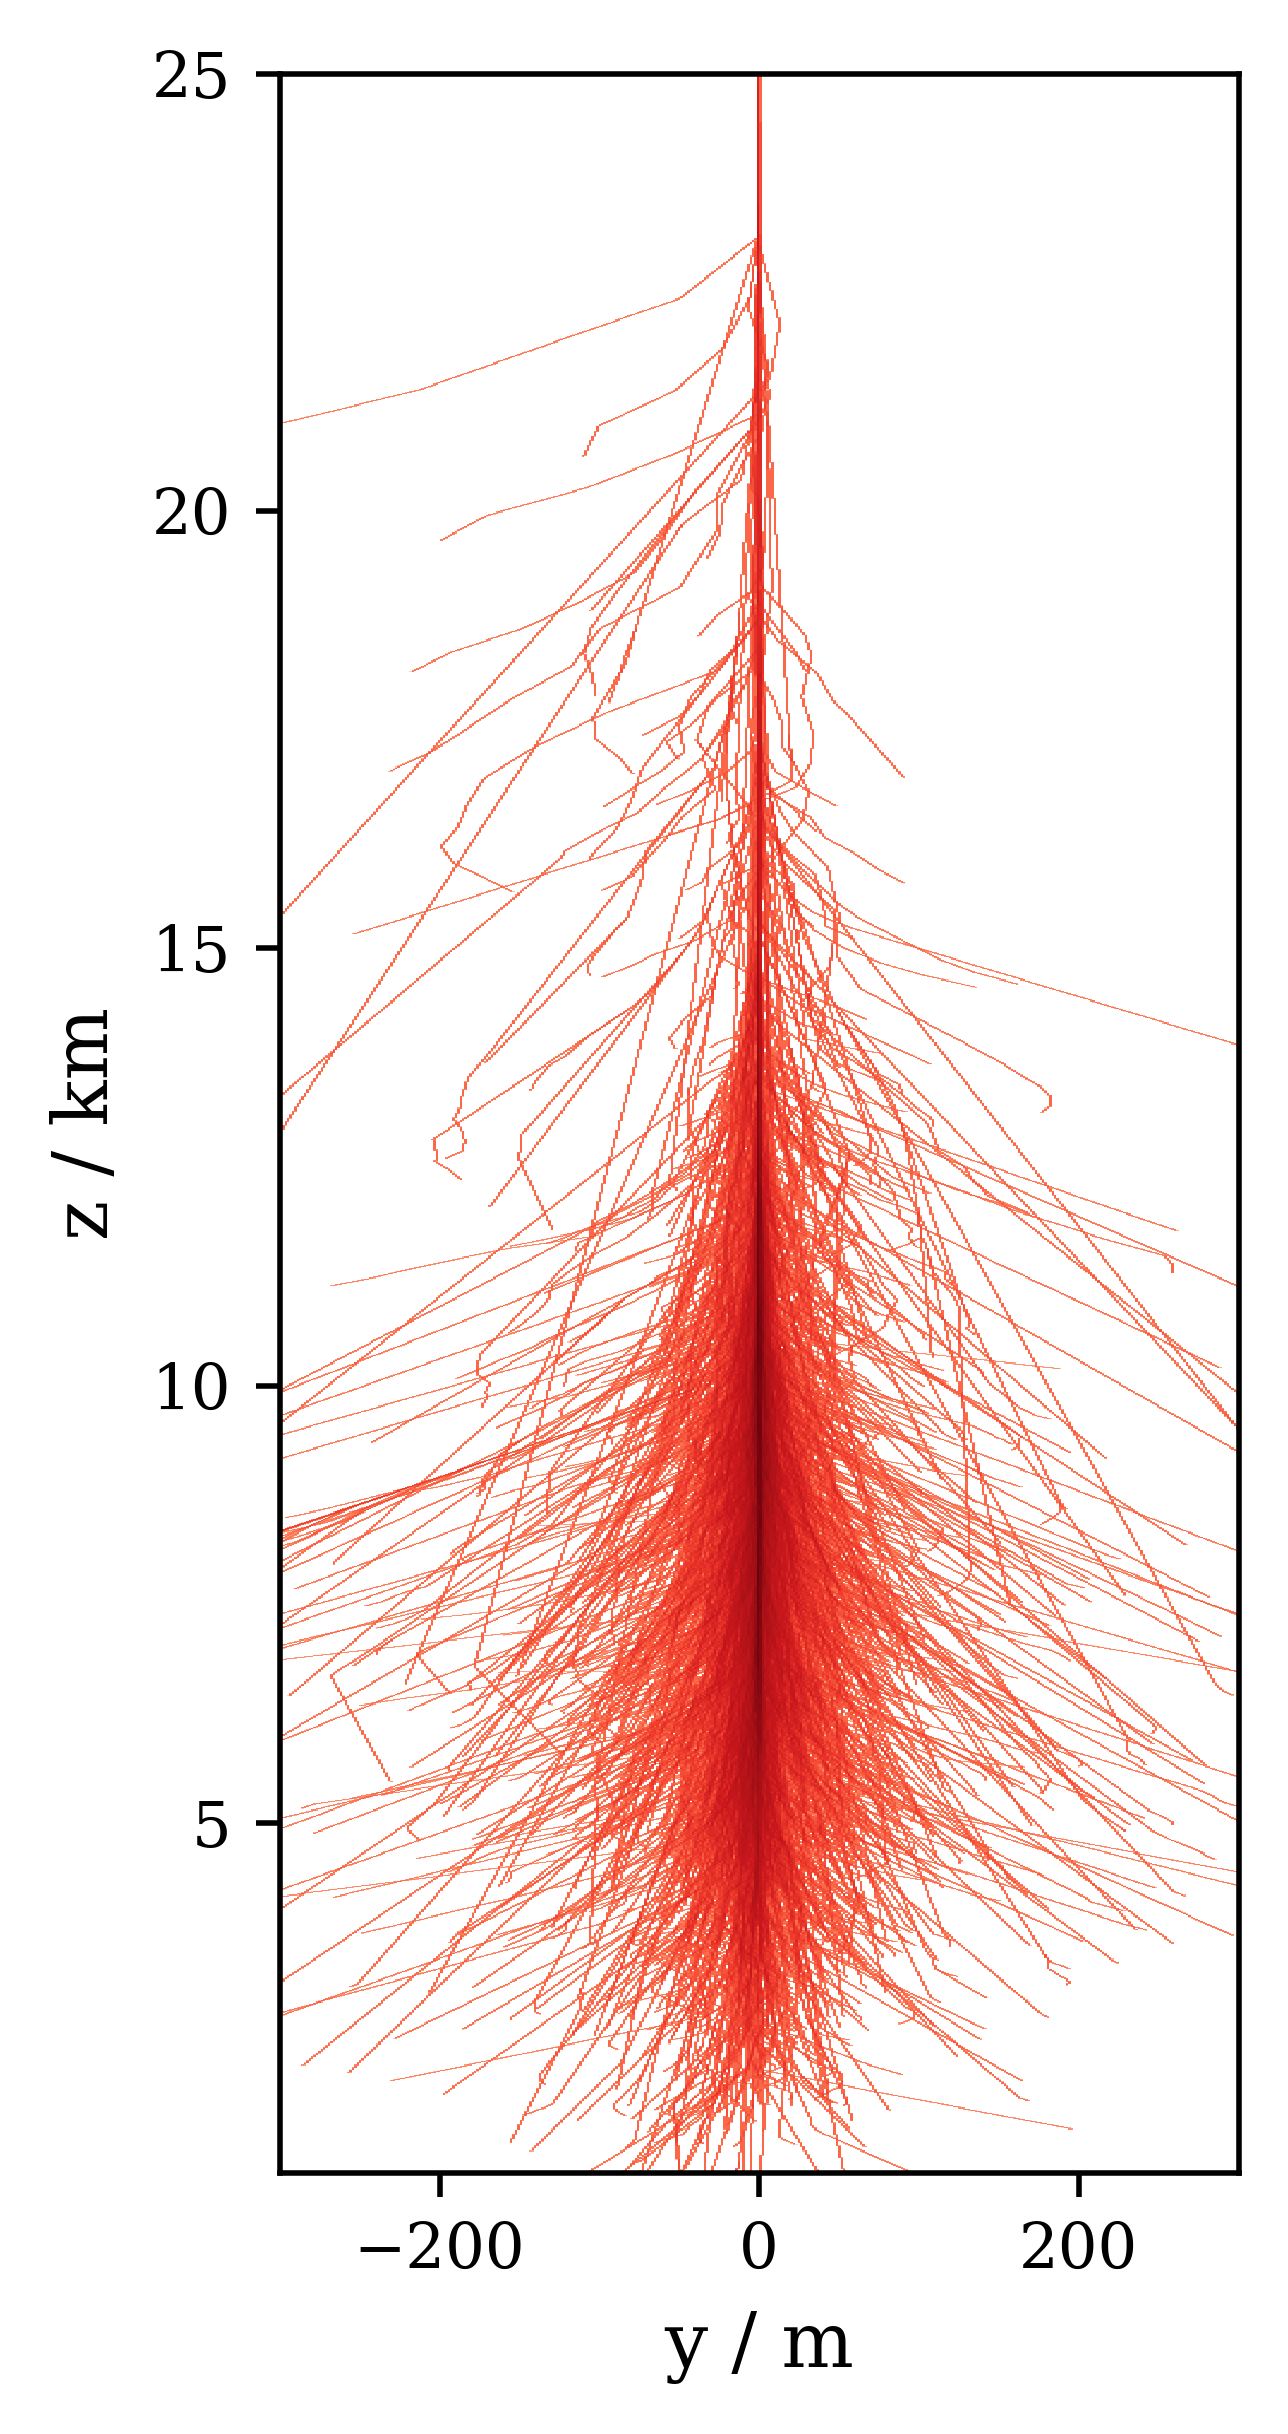
\includegraphics[width=0.75\linewidth, height=.4\textheight, keepaspectratio]{plots/shower.png}
                \caption*{\SI{1}{\tera\electronvolt} $e^-$ shower simulated with CORSIKA~8}
              \end{figure}
            \end{column}

          \end{columns}
      \end{block}%
    \end{column}%
    \begin{column}{0.4\textwidth}%
      \begin{block}[equal height group=B]{Application: Muography}%
        \begin{itemize}
          \setlength\itemsep{\itemseparation}
          \item Muography is a non-invasive imaging technique using Cosmic Ray muons
          \item Tracing the muon number along trajectories provides information, for example on density anomalies
          \item PROPOSAL is a well-suited tool to provide the necessary muon simulations
          \begin{itemize}
            \setlength\itemsep{\itemseparation}
            \item[$\rightarrow$] We are currently analyzing the possibilities to use muography in mining with PROPOSAL simulations
          \end{itemize} 
        \end{itemize}
      \vspace{3em}
        \begin{figure}
            \begin{tikzpicture}[scale=2.5, every node/.style={scale=0.85}]
                \centering

                \coordinate (A) at (0, 0);

                % ground
                \draw[draw=none, fill=gray, fill opacity=1.0] ($ (A) + (-3.5,-2.5) $) rectangle ++(7, 5);

                % sky
                \draw[draw=none, fill={rgb:red,0.33;green,0.5;blue,0.98}, fill opacity=0.5] ($ (A) + (-3.5,2.5) $) rectangle ++(7, 1);
                \node[draw=none] at ($ (A) + (0.0, 3) $) {Sky};

                % mining shaft
                \draw[draw=none, fill={rgb:black,1;white,2}, fill opacity=1.0] ($ (A) + (2, -1.5) $) rectangle ++(0.25, 4.0);
                \draw[draw=none, fill={rgb:black,1;white,2}, fill opacity=1.0] ($ (A) + (-2.0, -1.5) $) rectangle ++(4, 0.5);

                \node[draw=none] at ($ (A) + (0.8, -1.25) $) {Mining shaft};

                % detector
                \node [cylinder, shape border rotate=90, draw,minimum height=0.40cm,minimum width=0.25cm, aspect=0.4] (detector) at ($ (A) + (-0.5, -1.3) $) {};

                % impurity
                \draw[draw=none,fill=black, fill opacity=0.7] ($ (A) + (0, 0.07) $) ellipse (0.3cm and 0.1cm);
                \node[draw=none, text width=1cm] at ($ (A) + (0.9, 0.07) $) {Anomaly};

                % muons
                \draw [densely dotted, blue, line width=0.25mm] ($ (A) + (-2.5, 3.0) $) -- ($ (detector) + (0.2, -0.5) $) node [near start, above, xshift=1ex] (TextNode) {$\mu$};

                \draw [densely dotted, blue, line width=0.25mm] ($ (A) + (-1.0, 3.0) $) -- ($ (detector) + (0.1, -0.5) $) node [near start, above, xshift=1ex] (TextNode) {$\mu$};

                \draw [densely dotted, blue, line width=0.25mm] ($ (A) + (1.0, 3.0) $) -- ($ (A) + (0, 0.07) $) node [pos=0.4, above, xshift=-1ex] (TextNode) {$\mu$};

            \end{tikzpicture}
            \caption*{Visualization of the muography technique to explore density anomalies.}
        \end{figure} 

      \end{block}%
    \end{column}%
  \end{columns}%


  \vspace*{\fill}
  \begin{columns}[onlytextwidth]%
    \begin{column}{0.38\linewidth}%
      \begin{block}[equal height group=bottom, fonttitle=\normalsize]{References}
        \begin{multicols}{3}
          \footnotesize%
          \printbibliography%
        \end{multicols}
      \end{block}
    \end{column}
    \begin{column}{0.24\linewidth}%
      \begin{block}[equal height group=bottom, fonttitle=\normalsize]{Acknowledgements}
          We acknowledge funding by the Deutsche Forschungsgemeinschaft under the grant numbers XXXXX and SA 3876/2-1.\\
          Furthermore, this work has been supported by the DFG, Collaborative Research Center SFB 876 (project C3) and Collaborative Research Center SFB 1491.
      \end{block}
    \end{column}
    \begin{column}{0.38\linewidth}%
      \begin{block}[equal height group=bottom, fonttitle=\normalsize]{Contact}
        \begin{center}
  \begin{figure}[ht]
  \begin{minipage}[ht]{0.75\linewidth}
  \textbf{Find the PROPOSAL repository under:}\\ \url{github.com/tudo-astroparticlephysics/PROPOSAL}\\
  \vspace{0.2em}\\
  \textbf{Contact via mail:}\\ \href{mailto:me@jean-marco.alameddine@tu-dortmund.de}{jean-marco.alameddine@tu-dortmund.de} 

  \end{minipage}
    \begin{minipage}[ht]{0.24\linewidth}
    \centering
    
\includegraphics[%scale=1
                 width=0.95\linewidth, valign=t]{plots/qr_proposal.png}
    \end{minipage}
  \end{figure}
  \end{center}
  \end{block}
  \end{column}
  \end{columns}

  %\begin{block}[equal height group=bottom, fonttitle=\normalsize]{References}
  %  \begin{multicols}{3}
  %    \footnotesize%
  %    \printbibliography%
  %  \end{multicols}
  %\end{block}
\end{document}
